\documentclass{report}
\usepackage[margin=1in, paperwidth=8.5in, paperheight=11in]{geometry}
%Math packages%
\usepackage{amsmath}
\usepackage{amsthm}
%Spacing%
\usepackage{setspace}
\onehalfspacing
%Lecture number%
\newcommand{\lectureNum}{4}
%Variables - Date and Course%
\newcommand{\curDate}{January 12, 2017}
\newcommand{\course}{CS 240}
%Defining the example tag%
%\theoremstyle{definition}%
\newtheorem{ex}{Example}[section]
%Setting counter given the lecture number%
\setcounter{chapter}{\lectureNum{}}
%Package to insert code%
\usepackage{listings}
\usepackage{courier}
\usepackage{xcolor}
\lstset { 
    tabsize=2,
    breaklines=true,
    language=C++,
    backgroundcolor=\color{blue!8}, % set backgroundcolor
    basicstyle=\footnotesize\ttfamily,% basic font setting
}
%Package to draw trees%
\usepackage{tikz}

\begin{document}
%Note title%
\begin{center}
\begin{Large}
\textsc{\course{} | Lecture \lectureNum{}}
\end{Large}
\end{center} 
\noindent \textit{Bartosz Antczak} \hfill
\textit{Instructor: Eric Schost} \hfill
\textit{\curDate{}}
\rule{\textwidth}{0.4pt}

% Actual Notes%
\subsubsection{Today's plan}
\begin{itemize}
\item Wrap up loop analysis
\item Look at the merge sort algorithm
\item Introduce ourselves to heaps
\end{itemize}
\section{Wrapping up loop analysis}
\begin{ex}
Consider the following algorithm.
\end{ex}
\begin{lstlisting}
sum = 0
for (i = 1; i < n)
	j = i
	while (j >= 1)
		sum = sum + (i / j)
		j = floor(j/2)
return sum
\end{lstlisting}
For an integer $n$, let's call $b(n)$ the number of $digits$ of $n$ written in base 2 (e.g., $n=19=[10011]_2$, thus $b(n) = 5$).\\
We claim that $\log_2 (n) \leq b(n) \leq \log_2(n) + 2$ for all $n$. The proof is shown:\\
\textbf{Proof}:
\begin{align}
%Floor%
\lfloor \log_2 (n)\rfloor &\leq \log_2(n) \leq \lceil \log_2 (n)\rceil \\
2^{\lfloor \log_2 (n)\rfloor} &\leq n \leq 2^{\lceil \log_2 (n)\rceil}
\end{align}
Now note that $\lfloor \log_2 (n)\rfloor + 1 \leq b(2^{\lfloor \log_2 (n)\rfloor})$ and $b(2^{\lceil \log_2 (n)\rceil}) \leq \lceil \log_2 (n)\rceil + 1$
\begin{align}
\lfloor \log_2 (n)\rfloor + 1 &\leq b(n) \leq \lceil \log_2 (n)\rceil + 1 \\
(\log_2 (n) - 1) + 1 &\leq b(n) \leq  (\log_2 (n) + 1) + 1 \\
\log_2 (n) &\leq b(n) \leq  \log_2 (n) + 2
\end{align}
Now let's analyze the algorithm. For $i \geq 1$, let $u_3(i)$ be the number of times we enter the inner loop starting with $j=i$. Let $t_3(n)$ be the total runtime of the algorithm. Then $t_3(n) = \displaystyle \theta\left(\sum_{i=1}^n u_3(i)\right)$\\
By observation, we see that for each pass in the inner loop of the algorithm, it erases the last digit of $j$ in base 2. For instance, if $j=18=[10010]_2$, we see that $\lfloor \frac{j}{2} \rfloor = 9 = [1001]_2$.\\
Thus, $u_3(i) =$ the number of bits of $i$ written in base 2 $= b(i)$ (which is why we defined it previously).\\
Let's calculate it now:
\begin{align}
t_3(n) = \theta\left(\sum_{i=1}^n u_3(i)\right) = \sum_{i=1}^n b(i)\\
\log_2 (i) \leq b(i) \leq  \log_2 (i) + 2\\
\sum_{i=1}^n \log_2(i) \leq \sum_{i=1}^n b(i) \leq \sum_{i=1}^n \log_2(i) + \sum_{i=1}^n 2
\end{align}
Now referring to our cheat sheet on module 1, slide 38:
$$\sum_{i=1}^n \log_2(i) = \log_2\left(\prod_{i=1}^n i\right) = \log_2 (n!) \in \theta(n \log (n))$$
Therefore, $t_3(n) = \displaystyle\sum_{i=1}^n b(i) \in \theta(n \log_2(n))$.
\section{Design of MergeSort}
The recursive algorithm of mergesort receives an input an array $A$ of $n$ integers. The algorithm proceeds as follows:
\begin{itemize}
\item[1.] Split $A$ into two smaller arrays. Both arrays should contain the same number of elements or should differ by at most one (aka, split the array evenly or have at most one extra element in one subarray)
\item[2.] Recursively run MergeSort on both subarrays
\item[3.] After both subarrays have been sorted, use a function \texttt{Merge()} to merge them into a single sorted array
\end{itemize}
Mergesort has a runtime of $\theta(n)$.
The simplified algorithm structure of mergesort (\texttt{A, S, aL, aR} are arrays, and \texttt{n, nL, nR} are integer values):
\begin{lstlisting}
MergeSort(A, n) {
	if (n == 1) S = A
	else {
		nL = ceiling(n/2) // size of subarray 1
		nR = floor(n/2) // size of subarray 2
		aL = {A[1], ..., A[nL]} // subarray 1
		aR = {A[nL + 1], ..., A[n]} //subarray 2
		sL = MergeSort(aL, nL) // the sorted subarray 1
		sR = MergeSort(aR, nR) // the sorted subarray 2
		S = Merge(sL, nL, sR, nR) // The entire sorted array
	}
	return S
}
\end{lstlisting}
The 
\begin{center}
\textbf{| And this concludes Module 1: Order Notation |}.
\end{center} \newpage

%Module 2%
\section{Abstract Data Types}
An \textbf{Abstract Data Type (ADT)} is a description of information and a collection of operations on that information. The information is accessed only through the operations. We have various realizations (methods of implementation) of an ADT, which specify 
\begin{itemize}
\item How the information is stored (Data structure)
\item How operations are performed (algorithms)
\end{itemize}

\subsection{Priority Queue ADT}
A \textbf{priority queue} is an ADT consisting of a collection of items, where each item has a priority. An typical application of this is a ``todo" list. Two operations in a Priority Queue are
\begin{itemize}
\item \texttt{insert}: insert an item tagged with a priority
\item \texttt{deleteMax}: remove the item with the highest priority
\end{itemize}
\subsubsection{Possible Implementations of Priority Queues}
\begin{itemize}
\item[1.] Use an \textbf{unsorted array}. We see that the two operations have a runtime of
\begin{itemize}
\item \texttt{insert}: $O(1)$
\item \texttt{deleteMax}: $O(n)$
\end{itemize}
\item[2.] Use a \textbf{sorted array}. We see that the two operations have a runtime of
\begin{itemize}
\item \texttt{insert}: $O(n)$
\item \texttt{deleteMax}: $O(1)$
\end{itemize}
\item[3.] Use a \textit{heap} (defined in next subsection)
\end{itemize}
\subsection{Heaps}
A \textbf{heap} is a certain type of binary tree (recall that a binary tree is either empty or consists of three parts: a node, a left binary subtree and a right binary subtree).\\
Definition: a \textbf{max-heap} is a binary tree with the following two properties:
\begin{itemize}
\item \textbf{Structural Property}: all levels of a heap are completely filled, except maybe the last level. The filled items in the last level are \textit{left-justified} (for every node, their child on the left has their nodes filled with both children)
\item \textbf{Heap-order Property}: For any node $i$, the value of the parent of $i$ is larger than or equal to the value of $i$
\end{itemize}
Every node contains a value (or key).\newpage
\begin{ex}
Various trees that are and aren't heaps.
\end{ex}
%TREE #1 - THIS ONE IS A HEAP%
\begin{center}\begin{tikzpicture}[
  level distance=40 pt,
  every node/.style={circle,draw},
  level 1/.style={sibling distance=200 pt},
  level 2/.style={sibling distance=100 pt},
  level 3/.style={sibling distance=60 pt}
]
  \node {20}
    child {node {10}
      child {node {9}
      	child {node {6}}
      	child {node {6}}}
      child {node {7}
      	child {node {3}}
      	child [missing]}
    }
    child {node {19}
      child {node {2}}
      child {node {1}}
    };
\end{tikzpicture}\\Tree \# 1: A proper heap\\\end{center}
%TREE #2 - NOT A HEAP%
\begin{center}\begin{tikzpicture}[
  level distance=40 pt,
  every node/.style={circle,draw},
  level 1/.style={sibling distance=200 pt},
  level 2/.style={sibling distance=100 pt},
  level 3/.style={sibling distance=60 pt}
]
  \node {20}
    child {node {10}
      child {node {6}}
      child [missing]
    }
    child {node {19}
      child {node {2}}
      child [missing]
    };
\end{tikzpicture}
\\Tree \# 2: Not a heap (it's not left justified)\\\end{center}
%TREE #3 - NOT A HEAP%
\begin{center}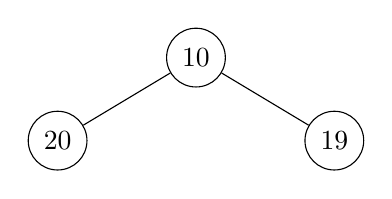
\begin{tikzpicture}[
  level distance=30 pt,
  every node/.style={circle,draw},
  level 1/.style={sibling distance=100 pt},
  level 2/.style={sibling distance=100 pt},
  level 3/.style={sibling distance=60 pt}
]
  \node {10}
    child {node {20}}
    child {node {19}};
\end{tikzpicture}
\\Tree \# 3: Not a heap (it doesn't follow the heap-order property)\end{center}
\subsubsection{Insertion in Heaps}
To insert a new node in a heap, we first place the new node at the first free leaf. However, this may violate the heap-order property, so we perform a \textit{bubble-up}.\\
A \textbf{bubble-up} is an algorithm that operates in the following way:
\begin{itemize}
\item While the parent of the new node exists and the value of the parent is less than the value of the new node, swap both nodes
\item The new node is now in its parent's position. Now repeat this algorithm
\end{itemize}
This algorithm has a runtime of $O(\log n)$\newpage
\subsubsection{Deleting in Heaps}
To delete the maximum item (node with the largest value), we replace the root with the last leaf (the rightmost child leaf in the lowest level of the tree). Again, this may violate the heap-order property, so we perform a \textit{bubble-down}.
A \textbf{bubble-down} is an algorithm that operates in the following way:
\begin{itemize}
\item While the replaced node is not a leaf, find the child node which has the largest value. If the value of the child is greater than the value of the replaced node, swap them. Otherwise, you're done.
\item If you swapped them, the replaced node is now in the position of its child node and the child node is now the parent node
\item Repeat this algorithm on the replaced node in its new position
\end{itemize}
This algorithm has a runtime of $O(\log n)$.
%END%
\end{document}